\subsection{Premières \routes{} \& \views{}}

\subsubsection[welcome!]{welcome!\label{sec:welcome!}}
Les \routes{} se trouvent dans le fichier \verb|routes\web.php|. \\
\begin{wrapfigure}[5]{r}{0.5\textwidth}
    \vspace{-0.5cm}
    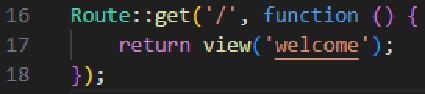
\includegraphics[width=0.5\textwidth]{figures-C1/basic_route.pdf}
\end{wrapfigure}
Dans ce fichier se trouve cette \route{} par défaut. Le premier argument de \verb|get()| est l'adresse (absolue) qui sera visée par la \route{}. En l'occurence, la fonction en deuxième argument sera exécutée lorsque l'URL est '/', donc \url{http://tutorialstepbystep/}. Remarquons que la fonction excécutée retourne la \view{} \textit{welcome}, c'est pourquoi nous voyons la page d'accueil de laravel en nous rendant à cette adresse.

Allons voir le contenu de cette \view{}. Les \views{} en \laravel{} ne sont pas écrites en fichier \verb|.html| classiques, mais sous la forme de fichiers \verb|fichier.blade.php|, qui permettent d'ajouter des fonctionnalités en plus\footnote{\textit{\underline{HINT:}} toutes les commandes commençant par un \verb|@| existent grâce au format \blade{}, ainsi que la commande \verb|{{}}|. Plus d'informations \href{https://laravel.com/docs/10.x/blade#blade-directives}{ici}.} à l'\html{} classique. 

Il y a bien beaucoup de chose dedans mais pas de panique: supprimons tout.

Plus précisément, ne gardons que ceci:

\begin{figure}[!h]
    \centering
    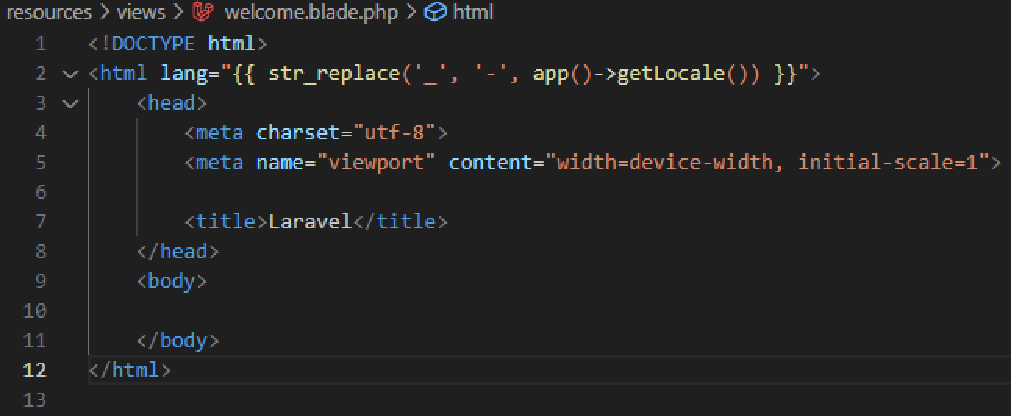
\includegraphics[width=0.75\textwidth]{figures-C1/welcome_blade_empty.pdf}
\end{figure}

On y voit déjà plus clair. Dans ce qu'il reste, il n'y a que deux choses principales à retenir pour le moment: 
\begin{enumerate}
    \item le tag \verb|<head>| est l'endroit où les styles (\css{}) et scripts (\jquery{}  \& \js{}) sont importés, ainsi que 2-{}3 autres choses.
    \item le tag \verb|<body>| est le tag qui contiendra tout ce qui sera affiché par le navigateur. Donc pour le moment, en allant sur votre site, vous verrez une page vide.
\end{enumerate}

\subsubsection[Controller][laravel.com/docs/10.x/controllers\#introduction]{Controller}

Bon, il est temps de remplir tout ca.

\begin{wrapfigure}[9]{r}{0.25\textwidth}
    \vspace{-0.5cm}
    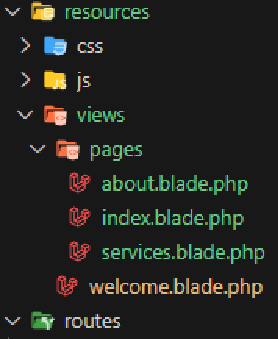
\includegraphics[width=0.25\textwidth]{figures-C1/3_premieres_views.pdf}
\end{wrapfigure}

Commençons par créer un fichier \verb|pages| dans \verb|resources/views/|, et ajoutez trois autres fichiers comme indiqué ci-contre.

Ensuite, il va falloir créer un \controller{}. Pour cela, tapez
\verb|sail artisan make:controller PagesController|\footnote{\verb|sail artisan make:| est une commande très utile pour créer énormément de fichiers que nous verrons plus tard. Comme nous l'utilisons au travers de \laravelsail, il faut utiliser \verb|sail artisan| à la place}. \linebreak Les \controllers{} se trouvent dans \verb|app\Http\controllers\|. Dans \verb|PagesController|, créez trois fonctions comme à la \textsc{Figure }\ref{fig:PagesController1}.

\SaveVerb{term}|PagesController|
\begin{figure}[!h]
    \centering
    \begin{subfigure}{0.49\textwidth}
        \centering
        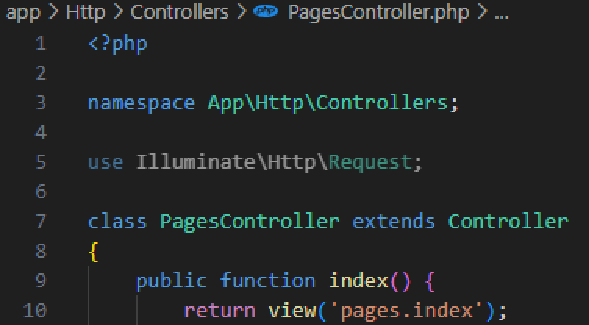
\includegraphics[width=\textwidth]{figures-C1/pages_controller_1a.pdf}
    \end{subfigure}
    \begin{subfigure}{0.49\textwidth}
        \centering
        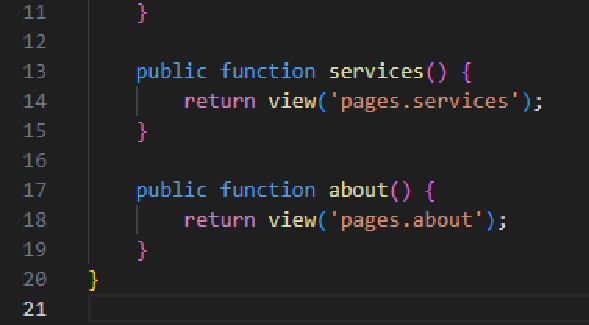
\includegraphics[width=\textwidth]{figures-C1/pages_controller_1b.pdf}
    \end{subfigure}
    \caption{\protect\UseVerb{term}\label{fig:PagesController1}}
\end{figure}

Vous l'aurez compris, \verb|return view()| permet d'afficher la \view{} donnée en argument: en l'occurence, les 3 \views{} \verb|index|, \verb|services| et \verb|about|. Notez que \verb|pages.| indique que ces 3 \views{} se trouvent dans le dossier \verb|pages|.

\newpage 

Si vous vous rappellez bien de ce qu'on a vu plus tôt, chaque \view{} \html{} doit contenir un tag \verb|<head>|. Celui-ci sera le même pour chaque page donc il serait judicieux\footnote{\textbf{D.R.Y}: \textit{Don't Repeat Yourself!}} de créer une sorte de template dans lequel on mettrait le \verb|<head>| et qui sera ensuite utilisé pour les 26854 pages que comptera bientôt notre site! 

COMME PAR HASARD les fichiers \verb|.blade.php| nous permettent de faire cela: commencez par créer un dossier \verb|layouts| dans les views, et créez un fichier dedans appellé \verb|app.blade.php|. Ensuite, remplissez-le avec le contenu de \verb|welcome.blade.php| (que vous pouvez désormais supprimer), puis ajoutez la commande \verb|@yield('content')| dans le \verb|<body>|. Enfin, il ne reste plus qu'a utiliser ce layout pour remplir vos 3 nouvelles \views{}.

\SaveVerb{about}|about|
\SaveVerb{services}|services|
\SaveVerb{index}|index|
\begin{figure}[!h]
    \centering
    \begin{subfigure}[b]{0.49\textwidth}
         \centering
         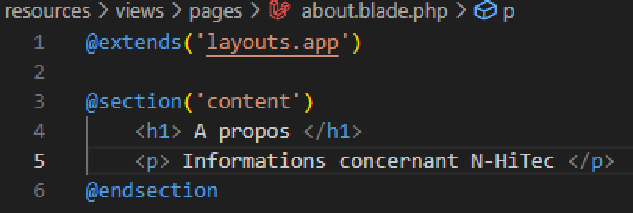
\includegraphics[width=\textwidth]{figures-C1/basic_about.pdf}
     \end{subfigure}
     \begin{subfigure}[b]{0.49\textwidth}
         \centering
         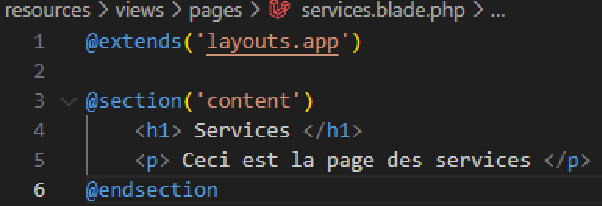
\includegraphics[width=\textwidth]{figures-C1/basic_services.pdf}
     \end{subfigure}
     \begin{subfigure}[b]{1\textwidth}
         \centering
         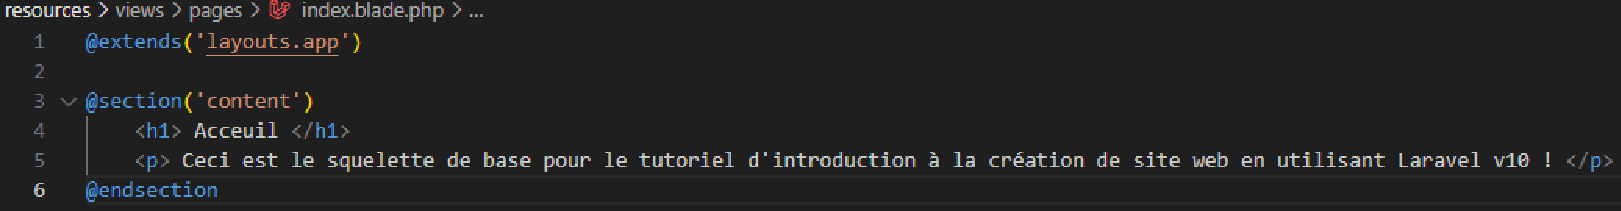
\includegraphics[width=\textwidth]{figures-C1/basic_accueil.pdf}
     \end{subfigure}
        \caption{Contenu des \views{} \protect\UseVerb{about} (à gauche), \protect\UseVerb{services} (à droite) et \protect\UseVerb{index} (en bas)}
\end{figure}
Petit tuto \html{} rapide: le tag \verb|<p>| renferme un pparagraphe, et le tag \verb|<h1>| contient lui un h1titre. De même, \verb|<h2>| désignera un h2sous-titre, \verb|<h3>| un h3sous-sous-titre, \verb|<h4>| un h4sous-sous-sous-titre, \ldots

Que se passe-t'il exactement? Chacune des \views{} va prendre le contenu du layout \verb|app| (via \verb|@extends()|), et remplir sa section \verb|content| par ce qu'il y a entre \verb|@section| et \verb|@endsection|. Simple et efficace! Nous rajouterons d'autres choses dans ce layout par la suite.

\newpage

Enfin, pour pouvoir admirer le fruit de votre dur labeur, il faut créer les \routes{} qui permettront d'afficher ces pages. Pour cela, rendez-vous dans \verb|web.php|:

\begin{wrapfigure}[16]{r}{0.7\textwidth}
    \vspace{-0.5cm}
    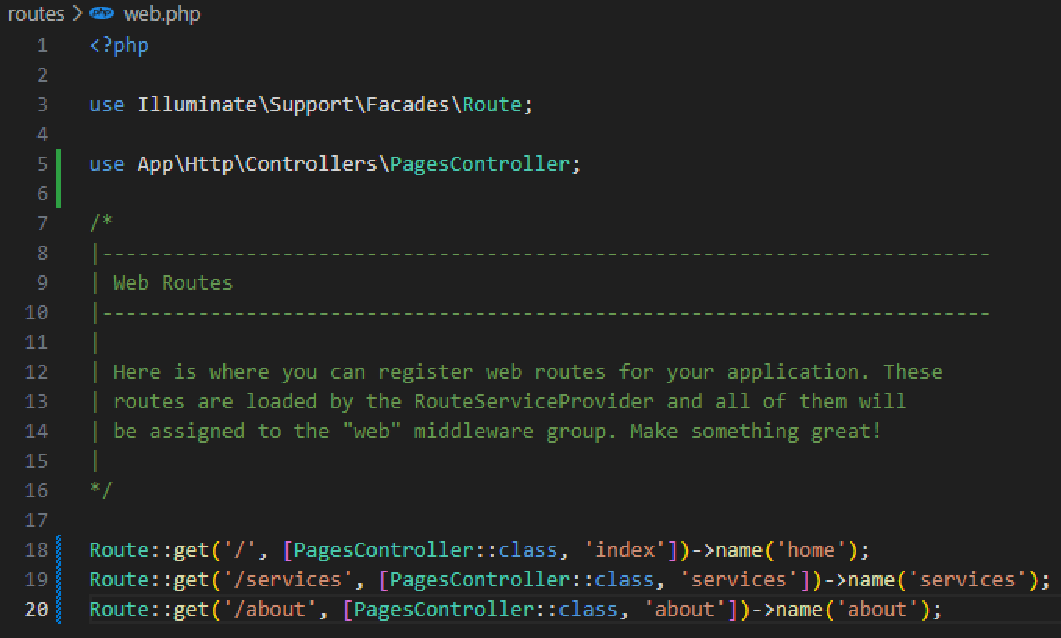
\includegraphics[width=0.7\textwidth]{figures-C1/3_premieres_routes.pdf}
    \caption{}
\end{wrapfigure}
Afin d'utiliser notre nouveau controller, il faut le déclarer pour que \laravel{} sache qu'il existe. C'est à ca que sert ``\verb|use gngngn|'', (ce qui est suit est plutôt évident).
Ensuite, décortiquons ce qui se passe: Comme précédement, le 1er argument de \verb|get()| donne l'adresse. Par exemple, la 2eme route est appellée à l'URL \url{http://tutorialstepbystep/services}. Le deuxième argument donne dans une \texttt{array} le \controller{} ainsi que sa méthode à exécuter. Pour la deuxième route, aller à l'URL mensionnée va donc exécuter la fonction \verb|services()| que nous avons créée il y a 5 (ou 40) minutes. Celle ci nous retourne la \view{} correspondante, donc en allant sur cet URL nous voyons dans un coin de l'écran:

\begin{figure}[!h]
    \centering
    \fbox{
\includegraphics[]{figures-C1/basic_services_web.pdf}}
    \caption{page internet moche}
\end{figure}

C'est laid, pas vrai? Nous allons améliorer cela à la prochaine section.

\newpage
